\begin{figure*}[!t]
\centering
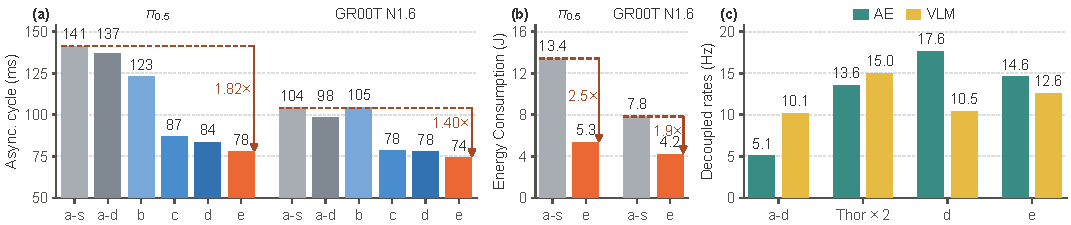
\includegraphics[width=\textwidth]{figures/evaluation-summary.pdf}
\caption{VLA-PIM evaluation.
(a) Asynchronous inference cycles for $\pi_{0.5}$ ($H=16$) and GR00T N1.6 ($H=15$).
a-s/a-d: serial/dual-stream GPU. b: PIM offloading. c: GPU--PIM concurrency.
d: dataflow optimization. e: full VLA-PIM.
For GR00T, the serial value sums separately measured phase means and the dual-stream value is median AE inference latency.
(b) Energy per AE chunk for the Thor GPU baseline (a-s) and full VLA-PIM (e).
Bar heights and labels give energy in joules. Each arrow is labeled with the ratio of Thor energy to VLA-PIM energy for that model.
Thor energy uses measured board input power and the steady AE completion period with a fresh KV cache.
VLA-PIM energy is estimated from a GPU power proxy, modeled DRAM and PIM logic power, and the duration of one simulated VLM--AE pair.
(c) Decoupled AE action-chunk and VLM KV-refresh rates for $\pi_{0.5}$.
The two loops share one GPU in a-d and run on dedicated GPUs in Thor~$\times$~2.
VLA-PIM (d) streams inputs and (e) preloads them.}
\label{fig:evaluation-summary}
\end{figure*}
